% Koma class
\documentclass[a4paper, oneside]{scrartcl}   

\usepackage{a4wide}

%------------------
% language = english
\usepackage[english, german]{babel}	% Umlaute mit \"u
\usepackage[latin1]{inputenc}

% margins + Kopf- und Fu�zeilen
\usepackage[left = 2.5cm, right = 2.5cm, top = 2cm, bottom = 3cm]{geometry}
\usepackage{scrpage2} 
\pagestyle{scrheadings}
\clearscrheadfoot
\rehead{\headmark}
\lehead{\pagemark}
\lohead{\headmark}
\rohead{\pagemark} 


% math
\usepackage{amssymb}
\usepackage{amsmath}

% figures
\usepackage{tikz}
\usepackage{graphicx}


% section-Zaehler wird neu gesetzt:
\setcounter{section}{3}
%------------------
\author{Sascha Meiers, Martin Seeger}
\title{Exercise 3, Discrete Mathematics for Bioinformatics}
\date{Winter term 2011/2012}


\begin{document}
\maketitle

%---------------------------------------------------------------------------------------------------

\subsection{Skip lists}

\noindent a) Expected value of $h$ (adapted from script): 
we use the notation from the script:
$x\in S$, $h(x) =$ number of sets $S_i$ containing $x$, $h = 1+\max\{h(x):
x\in S\}$. 

For $k\geq 1$, we have $P(h(x) \geq k) = p^{k-1}$ and therefore 
\[
P(h \geq k+1) = nP(h(x) \geq k) = np^{k-1}.
\]
This estimate does not make sense for $k < 1 + \log_{1/p} n=1 - \log_{p} n$.
For those values of $k$ we can use the trivial upper bound $P(h \geq k+1) \leq 
1$. Then $E(h)$ equals:
\begin{eqnarray}
\sum_{k=1}^\infty P(h \geq k+1) &=& \sum_{k=1}^{\lceil - \log_{p} n \rceil} P(h
\geq k+1)+\sum_{k=1+\lceil - \log_{p} n \rceil}^{\infty} P(h \geq k+1) 
\leq \nonumber \\
&\leq& 1+\lceil - \log_{p} n \rceil + \sum_{k=1+\lceil - \log_{p} n
\rceil}^{\infty} np^{k-1}=
\nonumber \\
&=& 1+\lceil - \log_{p} n \rceil + \frac{n p^{\lceil - \log_{p} n \rceil}}{1-p}
= \nonumber \\
&\leq& 1+\lceil - \log_{p} n \rceil + \frac{n p^{- \log_{p} n}}{1-p} =
\nonumber \\
&=& 1+\lceil - \log_{p} n \rceil + \frac{1}{1-p}.
\nonumber 
\end{eqnarray}
For $p=1/3$ this yields $E(h) \leq 5/2+\lceil \log_{3} n \rceil$.
\\

\noindent b) Expected value of space consumption (adapted from script):
let M denote the total size of the sets $S_1,S_2, ... ,S_h$.
Then $M = \sum_{x\in S} h(x)$ and by linearity of expectation:
\begin{eqnarray}
E(M) = \sum_{x\in S} E(h(x)) = \frac{n}{p}.
\nonumber
\end{eqnarray}
We need to add the $h$ pseudo nodes at $-\infty$, so that the total size is
\[
E(M) + E(h) \leq \frac{n}{p} + 1+\lceil - \log_{p} n \rceil + \frac{1}{1-p}.
\]
For $p=1/3$ this yields $E(M) + E(h) \leq 3n + 5/2+\lceil \log_{3} n \rceil$.
\\

\noindent c) Expected value of search time (adapted from script):
Let $x$ be a real number and let $C_i$ denote the number of elements in the list 
$L_i$ that are inspected when searching for $x$. (We do not count the element of
$L_i$ at which the algorithm starts walking to the right. Hence, $C_i$ counts
comparisons between $x$ and elements of $S$.) The search cost is then
proportional to $\sum_{i=1}^h (1+C_i)$.

We first estimate the search level above $A$, i.e., the total costs in the lists 
$L_{A+1}, L_{A+2}, ... , L_h$. Since the cost is at most equal to the total size
of these lists, its expected value is at most equal to the expected value of
$M_A := \sum_{i=A+1}^h |L_i|$.

We can write
\[
E(M_A) = \sum_{k=0}^n E(M_A||S_{A+1}|=k)P(|S_{A+1}|=k),
\]
where
\[
E(M_A||S_{A+1}|=k) = 2k,
\]
and
\[
P(|S_{A+1}|=k) = {n \choose k} p^{Ak} (1-p^A)^{n-k}.
\]
Therefore
\[
E(M_A) = 2 \sum_{k=0}^n k {n \choose k} p^{Ak} (1-p^A)^{n-k} = 2np^A,
\]
for lists above $A$.

For lists up to $A$, we consider
\[
E(C_i) = \sum_{k=1}^n E(C_i|l_i(x)=k)P(l_i(x)=k),
\]
where $l_i(x)$ is the number of elements in $L_i$ that are $\leq x$.

We have for the first term
\[
E(C_i|l_i(x)=k) = \sum_j j P(C_i=j|l_i(x)=k) \leq \sum_j j p^{j-1} = (1-p)^{-2}
\]
independently of $k$ whence follows that
\[
E(C_i) \leq (1-p)^{-2} \sum_{k=1}^n P(l_i(x)=k) = (1-p)^{-2}.
\]
For the search cost up to $A$ we obtain
\[
E\left(\sum_{i=1}^A(1+C_i)\right) \leq A (1 + (1-p)^{-2}).
\]
Adding up, this yields total expected cost
\[
E\left(\sum_{i=1}^A(1+C_i)\right) + E(M_A) \leq A (1 + (1-p)^{-2}) + 2np^A.
\]
Using $A = \log_{1/p} n$, this becomes
\[
E\left(\sum_{i=1}^A(1+C_i)\right) + E(M_A) \leq (1 + (1-p)^{-2}) \log_{1/p} n +
2,
\]
and setting $p=1/3$, we find
\[
E\left(\sum_{i=1}^A(1+C_i)\right) + E(M_A) \leq \frac{13}{4} \log_{3} n +
2.
\]
\\



Remember that for each element in $S$ we throw a coin until $0$ comes up and count the number of coin throws which resulted in $1$. The probabilities are given with $Pr(1)= 1/3$ and therefore $Pr(0)=2/3$. The expected value of a geometric distribution is defined as $E(x)=1/p$. Which results in an expected value for $h$ of $1/(2/3) = 1.5$.


\subsection{``Sparse'' skip list}

We can drop the left--ingoing edges of all nodes that have a top--ingoing edge without affecting the search algorithm.
Searching for element 10 (which is not in the list) walks the same path as before ($-\infty, -\infty, -\infty, 2,5,5,8,8,9$). 
The only difference is that element 9 has no further pointer, which ends the search unsuccessfully, 
instead of pointing to 11 which also ends the search successfully.

\begin{figure}[h]
\centering
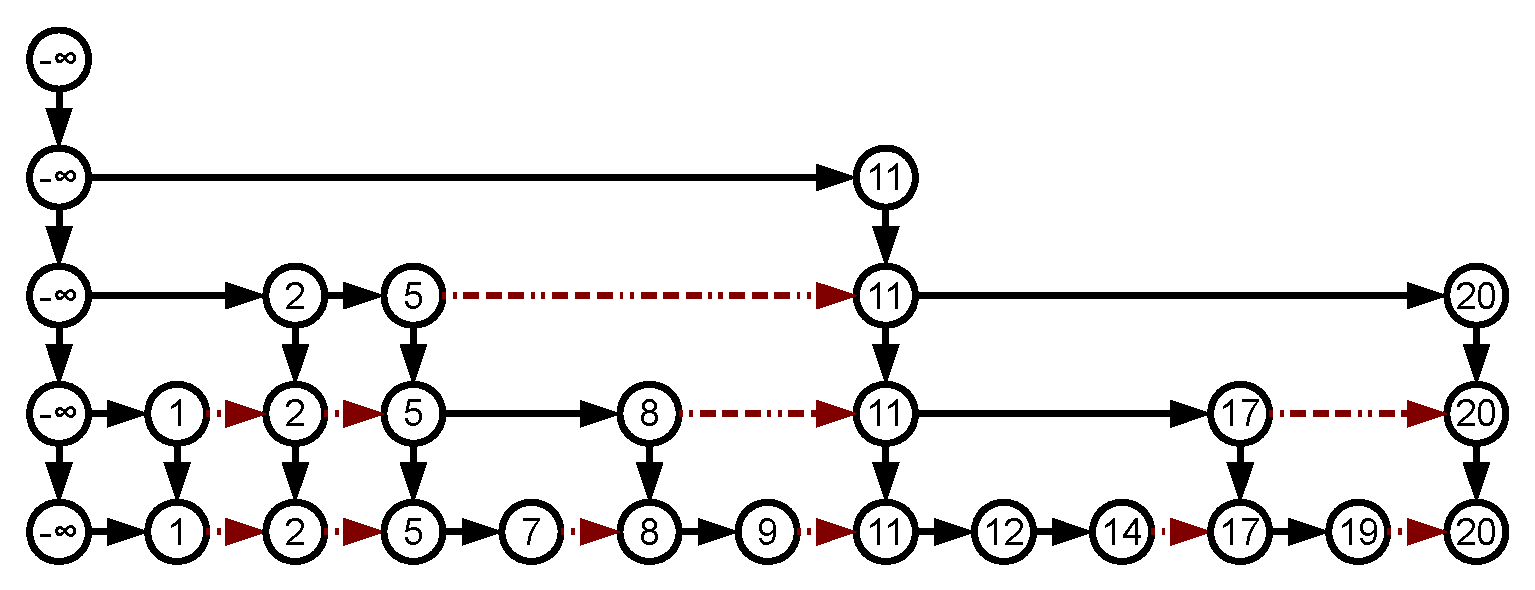
\includegraphics[width=\textwidth]{Skiplist.pdf}
\caption{Shown here is the skip list example from the script. The dotted red edges can be removed without affecting the search algorithm.}
\label{fig:SkipList}
\end{figure}

As shown in the figure, the number of edges we can remove per column is the height of the column minus one. 
Using the expected value for the height $h(x)$, we can derive he overall number of redundant edges: \[ n \cdot E(h(x)-1) =  n \left(E(h(x)) - 1 \right) = n\]

Remark: We think that in practice leaving out these edges brings no advantage for the algorithm, because an element may contain only one pointer instead of two, but it nevertheless has to memorize whether this pointer is a right--pointer or a down--pointer and in case of an appropriate insertion event, the second pointer has to be added. So in fact each element has to allocate the memory for both pointers, even if one is not used.

\subsection{Skip lists}

\paragraph{a)} First we will reconcider a part of the proof in the script:
\begin{align}
E(h) &= \sum\limits_{k=1}^\infty k \cdot Pr(h = k) \\
&= \begin{array}{cccc} Pr(h=1) + & & & \\ Pr(h=2) + & Pr(h=2) + & & \\ Pr(h=3) + & Pr(h=3) + & Pr(h=3) + & \\ \vdots & & & \end{array} \\
&= Pr(h \geq 1) +  Pr(h \geq 2) +  Pr(h \geq 3) +  \ldots  \\
&= \sum\limits_{k=0}^\infty Pr(h \geq k+1)
\end{align}
The probability that the height $h$ of a skip list is larger than $k$ is bounded by
\[ Pr(h\geq k+1) \leq n \cdot Pr(h(x) \geq k) = n \cdot \frac{1}{2^{k-1}} \]
So the probability that $h \geq c \cdot log\;n +1$ (so nearly $c$-times the expected value) is
\[ n \cdot \frac{1}{2^{c \cdot log\;n-1}} = \frac{2n}{n^{c}}  = \frac{2}{n^{c-1}} \]



\subsection{Independencies}

\paragraph {a)}
Let $\Omega_x, \Omega_y$ be the sets of elementary events of two different discrete random events 
(e.g. a coin throw and the color in a game of Roulette). 
Additionally, let $X: \Omega_x \to \mathbb{R}, Y: \Omega_y \to \mathbb{R}$ 
random variables for both experiments. The expected values of those random variables are
\[
E(X) = \sum\limits_{x \in \Omega_x} Pr(x) \cdot X(x) \qquad  
E(Y) = \sum\limits_{y \in \Omega_y} Pr(y) \cdot Y(y)  
\]

\begin{align}
E(X+Y)  &= \sum\limits_{x \in \Omega_x} \sum\limits_{y \in \Omega_y} Pr(x,y) \cdot (X(x) + Y(y))    \\
        &= \sum\limits_{x \in \Omega_x} \sum\limits_{y \in \Omega_y} Pr(x,y) X(x) + Pr(x,y) Y(y)    \\
        &= \sum\limits_{x \in \Omega_x} X(x) \underbrace{\sum\limits_{y \in \Omega_y} Pr(x,y) }_{Pr(x)} 
         + \sum\limits_{y \in \Omega_y} Y(y) \underbrace{\sum\limits_{x \in \Omega_x} Pr(x,y) }_{Pr(y)} \\
        &= E(X) + E(Y)
\end{align}

\begin{align}
E(X\cdot Y)  &= \sum\limits_{x \in \Omega_x} \sum\limits_{y \in \Omega_y} Pr(x,y) \cdot X(x) \cdot  Y(y)    \\
             &= \sum\limits_{x \in \Omega_x} \sum\limits_{y \in \Omega_y} Pr(x)\cdot Pr(y) \cdot X(x) \cdot  Y(y)    \\
             &= \sum\limits_{x \in \Omega_x} Pr(x)\cdot X(x)  \cdot \sum\limits_{y \in \Omega_y}  Pr(y) \cdot  Y(y)    \\
             &= E(X) \cdot E(Y)
\end{align}
In (10) we use the independence of $X$ and $Y$.

\paragraph {b)}
We have
\[
E(X_1) = \frac{1}{9}(1+1+2+2+3+3+1+2+3) = 2,
\]
\[
E(X_2) = \frac{1}{9}(2+3+1+3+1+2+1+2+3) = 2,
\]
\[
E(X_3) = \frac{1}{9}(3+2+3+1+2+1+1+2+3) = 2.
\]

\paragraph{i} Counting all the cases leads to $Pr(X_i = r) = \frac{3}{9} = \frac{1}{3}$ for $i=1,2,3$ and $r=1,2,3$

\paragraph{ii} $Pr(X_1=r \wedge X_2 = s) = \frac{1}{9}$ by counting all the cases for arbitrary $r,s$.  \\
This is equal to $Pr(X_1=r) \cdot  Pr(X_2 = s)$. Same for the random variables $X_1,X_3$ and 
$X_2,X_3$.

\paragraph{iii} Counter example: $Pr(X_1 = 1 \wedge X_2 = 1 \wedge X_3 = 1) = \frac{1}{9}$, which is not equal to \\
$Pr(X_1 = 1) \cdot Pr(X_2 = 1) \cdot Pr(X_3 = 1) = \frac{1}{3} \cdot \frac{1}{3} \cdot \frac{1}{3} = \frac{1}{27}$.

\paragraph{iv}  $E(N) = E(X_2) = 2$ as shown above.

\paragraph{v} Since $E(N)$ is not a random variable, we can simply plug in $E(N) = 2$:
            \[ \sum_{i=1}^{E(N)} E(X_i) = E(X_1) + E(X_2) = 4. \]

\paragraph{vi} 
\begin{eqnarray}
E\left(\sum_{i=1}^{N} X_i\right)&=& 
P(N=1)E\left(\sum_{i=1}^{1} X_i\middle| N=1\right)+
P(N=2)E\left(\sum_{i=1}^{2} X_i\middle| N=2\right)+
\nonumber \\
&+&P(N=3)E\left(\sum_{i=1}^{3} X_i\middle| N=3\right)=
\frac{2}{3}+
\frac{2+2}{3}+
\frac{2+2+3}{3}=\frac{13}{3}.
\nonumber 
\end{eqnarray}

\end{document}
